% Created by tikzDevice version 0.12.6 on 2025-04-16 10:40:07
% !TEX encoding = UTF-8 Unicode
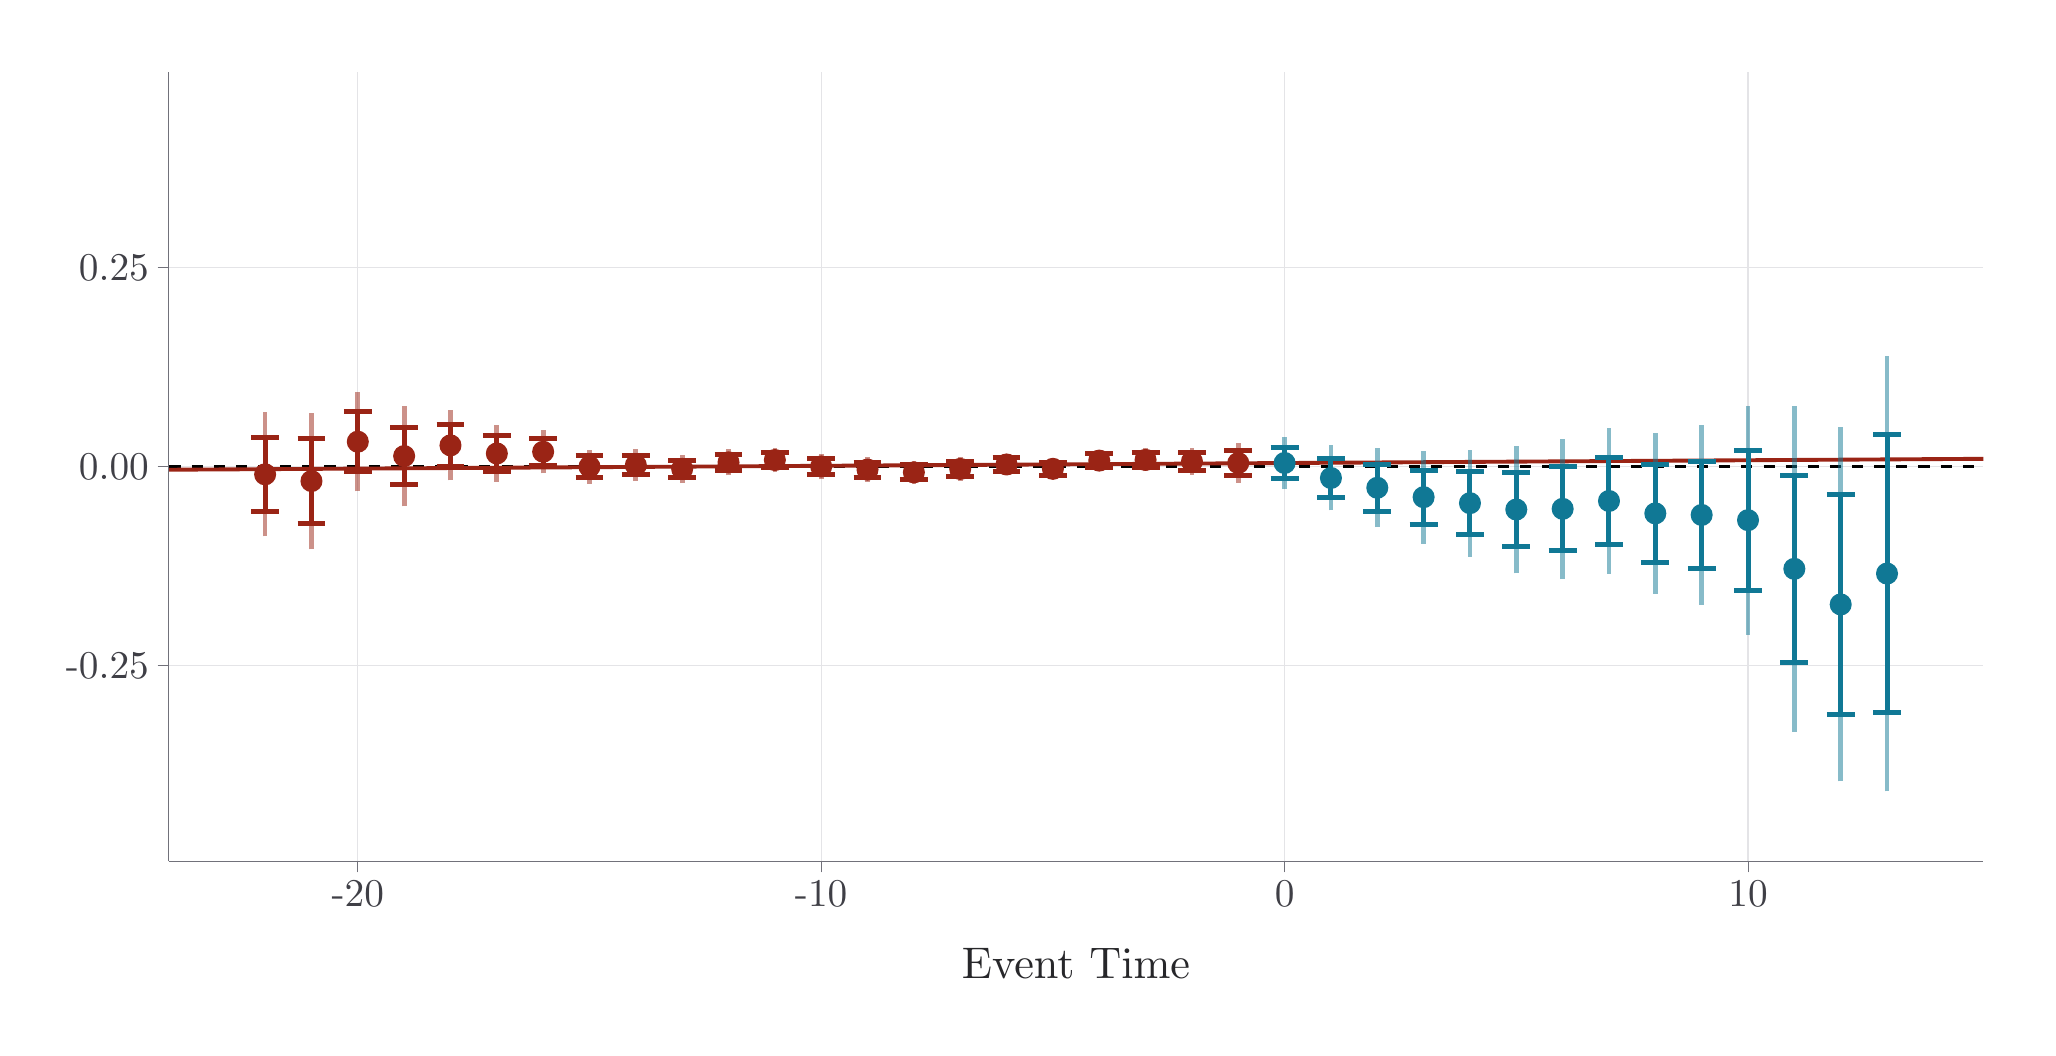
\begin{tikzpicture}[x=1pt,y=1pt]
\definecolor{fillColor}{RGB}{255,255,255}
\path[use as bounding box,fill=fillColor] (0,0) rectangle (722.70,361.35);
\begin{scope}
\path[clip] (  0.00,  0.00) rectangle (722.70,361.35);
\definecolor{drawColor}{RGB}{255,255,255}

\path[draw=drawColor,line width= 0.8pt,line join=round,line cap=round,fill=fillColor] (  0.00,  0.00) rectangle (722.70,361.35);
\end{scope}
\begin{scope}
\path[clip] ( 50.97, 60.16) rectangle (706.70,345.35);
\definecolor{drawColor}{RGB}{255,255,255}
\definecolor{fillColor}{RGB}{255,255,255}

\path[draw=drawColor,line width= 0.8pt,line join=round,line cap=round,fill=fillColor] ( 50.97, 60.16) rectangle (706.70,345.35);
\definecolor{drawColor}{RGB}{228,228,231}

\path[draw=drawColor,line width= 0.4pt,line join=round] ( 50.97,130.73) --
	(706.70,130.73);

\path[draw=drawColor,line width= 0.4pt,line join=round] ( 50.97,202.75) --
	(706.70,202.75);

\path[draw=drawColor,line width= 0.4pt,line join=round] ( 50.97,274.77) --
	(706.70,274.77);

\path[draw=drawColor,line width= 0.4pt,line join=round] (119.29, 60.16) --
	(119.29,345.35);

\path[draw=drawColor,line width= 0.4pt,line join=round] (286.74, 60.16) --
	(286.74,345.35);

\path[draw=drawColor,line width= 0.4pt,line join=round] (454.19, 60.16) --
	(454.19,345.35);

\path[draw=drawColor,line width= 0.4pt,line join=round] (621.64, 60.16) --
	(621.64,345.35);
\definecolor{drawColor}{RGB}{0,0,0}

\path[draw=drawColor,line width= 0.9pt,dash pattern=on 4pt off 4pt ,line join=round] (-604.76,202.75) -- (1362.43,202.75);
\definecolor{drawColor}{RGB}{154,36,21}

\path[draw=drawColor,line width= 1.4pt,line join=round] (-604.76,197.66) -- (1362.43,209.50);
\definecolor{drawColor}{RGB}{154,36,21}

\path[draw=drawColor,draw opacity=0.50,line width= 1.7pt,line join=round] ( 85.80,177.52) -- ( 85.80,222.37);

\path[draw=drawColor,draw opacity=0.50,line width= 1.7pt,line join=round] (102.55,172.85) -- (102.55,222.19);

\path[draw=drawColor,draw opacity=0.50,line width= 1.7pt,line join=round] (119.29,193.79) -- (119.29,229.70);

\path[draw=drawColor,draw opacity=0.50,line width= 1.7pt,line join=round] (136.04,188.33) -- (136.04,224.74);

\path[draw=drawColor,draw opacity=0.50,line width= 1.7pt,line join=round] (152.78,197.75) -- (152.78,223.07);

\path[draw=drawColor,draw opacity=0.50,line width= 1.7pt,line join=round] (169.53,197.32) -- (169.53,217.64);

\path[draw=drawColor,draw opacity=0.50,line width= 1.7pt,line join=round] (186.27,200.33) -- (186.27,215.89);

\path[draw=drawColor,draw opacity=0.50,line width= 1.7pt,line join=round] (203.01,196.57) -- (203.01,208.86);

\path[draw=drawColor,draw opacity=0.50,line width= 1.7pt,line join=round] (219.76,197.47) -- (219.76,209.00);

\path[draw=drawColor,draw opacity=0.50,line width= 1.7pt,line join=round] (236.50,196.76) -- (236.50,207.07);

\path[draw=drawColor,draw opacity=0.50,line width= 1.7pt,line join=round] (253.25,199.55) -- (253.25,208.98);

\path[draw=drawColor,draw opacity=0.50,line width= 1.7pt,line join=round] (269.99,200.68) -- (269.99,209.56);

\path[draw=drawColor,draw opacity=0.50,line width= 1.7pt,line join=round] (286.74,198.13) -- (286.74,207.44);

\path[draw=drawColor,draw opacity=0.50,line width= 1.7pt,line join=round] (303.48,197.23) -- (303.48,206.10);

\path[draw=drawColor,draw opacity=0.50,line width= 1.7pt,line join=round] (320.23,196.43) -- (320.23,204.87);

\path[draw=drawColor,draw opacity=0.50,line width= 1.7pt,line join=round] (336.97,197.67) -- (336.97,206.13);

\path[draw=drawColor,draw opacity=0.50,line width= 1.7pt,line join=round] (353.72,199.56) -- (353.72,207.46);

\path[draw=drawColor,draw opacity=0.50,line width= 1.7pt,line join=round] (370.46,198.31) -- (370.46,205.55);

\path[draw=drawColor,draw opacity=0.50,line width= 1.7pt,line join=round] (387.21,201.04) -- (387.21,208.78);

\path[draw=drawColor,draw opacity=0.50,line width= 1.7pt,line join=round] (403.95,200.99) -- (403.95,209.33);

\path[draw=drawColor,draw opacity=0.50,line width= 1.7pt,line join=round] (420.70,199.80) -- (420.70,209.39);

\path[draw=drawColor,draw opacity=0.50,line width= 1.7pt,line join=round] (437.44,196.95) -- (437.44,211.11);
\definecolor{drawColor}{RGB}{16,120,149}

\path[draw=drawColor,draw opacity=0.50,line width= 1.7pt,line join=round] (454.19,194.57) -- (454.19,213.54);

\path[draw=drawColor,draw opacity=0.50,line width= 1.7pt,line join=round] (470.93,186.88) -- (470.93,210.38);

\path[draw=drawColor,draw opacity=0.50,line width= 1.7pt,line join=round] (487.68,180.85) -- (487.68,209.34);

\path[draw=drawColor,draw opacity=0.50,line width= 1.7pt,line join=round] (504.42,174.89) -- (504.42,208.49);

\path[draw=drawColor,draw opacity=0.50,line width= 1.7pt,line join=round] (521.17,170.18) -- (521.17,208.88);

\path[draw=drawColor,draw opacity=0.50,line width= 1.7pt,line join=round] (537.91,164.18) -- (537.91,210.28);

\path[draw=drawColor,draw opacity=0.50,line width= 1.7pt,line join=round] (554.66,162.08) -- (554.66,212.88);

\path[draw=drawColor,draw opacity=0.50,line width= 1.7pt,line join=round] (571.40,164.01) -- (571.40,216.62);

\path[draw=drawColor,draw opacity=0.50,line width= 1.7pt,line join=round] (588.15,156.73) -- (588.15,214.93);

\path[draw=drawColor,draw opacity=0.50,line width= 1.7pt,line join=round] (604.89,152.90) -- (604.89,217.64);

\path[draw=drawColor,draw opacity=0.50,line width= 1.7pt,line join=round] (621.64,141.99) -- (621.64,224.78);

\path[draw=drawColor,draw opacity=0.50,line width= 1.7pt,line join=round] (638.38,107.02) -- (638.38,224.57);

\path[draw=drawColor,draw opacity=0.50,line width= 1.7pt,line join=round] (655.13, 88.96) -- (655.13,216.90);

\path[draw=drawColor,draw opacity=0.50,line width= 1.7pt,line join=round] (671.87, 85.36) -- (671.87,242.81);
\definecolor{drawColor}{RGB}{154,36,21}

\path[draw=drawColor,line width= 1.8pt,line join=round] ( 80.78,213.31) --
	( 90.82,213.31);

\path[draw=drawColor,line width= 1.8pt,line join=round] ( 85.80,213.31) --
	( 85.80,186.58);

\path[draw=drawColor,line width= 1.8pt,line join=round] ( 80.78,186.58) --
	( 90.82,186.58);

\path[draw=drawColor,line width= 1.8pt,line join=round] ( 97.52,213.02) --
	(107.57,213.02);

\path[draw=drawColor,line width= 1.8pt,line join=round] (102.55,213.02) --
	(102.55,182.02);

\path[draw=drawColor,line width= 1.8pt,line join=round] ( 97.52,182.02) --
	(107.57,182.02);

\path[draw=drawColor,line width= 1.8pt,line join=round] (114.27,222.58) --
	(124.31,222.58);

\path[draw=drawColor,line width= 1.8pt,line join=round] (119.29,222.58) --
	(119.29,200.91);

\path[draw=drawColor,line width= 1.8pt,line join=round] (114.27,200.91) --
	(124.31,200.91);

\path[draw=drawColor,line width= 1.8pt,line join=round] (131.01,216.97) --
	(141.06,216.97);

\path[draw=drawColor,line width= 1.8pt,line join=round] (136.04,216.97) --
	(136.04,196.11);

\path[draw=drawColor,line width= 1.8pt,line join=round] (131.01,196.11) --
	(141.06,196.11);

\path[draw=drawColor,line width= 1.8pt,line join=round] (147.76,217.94) --
	(157.80,217.94);

\path[draw=drawColor,line width= 1.8pt,line join=round] (152.78,217.94) --
	(152.78,202.88);

\path[draw=drawColor,line width= 1.8pt,line join=round] (147.76,202.88) --
	(157.80,202.88);

\path[draw=drawColor,line width= 1.8pt,line join=round] (164.50,213.98) --
	(174.55,213.98);

\path[draw=drawColor,line width= 1.8pt,line join=round] (169.53,213.98) --
	(169.53,200.98);

\path[draw=drawColor,line width= 1.8pt,line join=round] (164.50,200.98) --
	(174.55,200.98);

\path[draw=drawColor,line width= 1.8pt,line join=round] (181.25,213.07) --
	(191.29,213.07);

\path[draw=drawColor,line width= 1.8pt,line join=round] (186.27,213.07) --
	(186.27,203.15);

\path[draw=drawColor,line width= 1.8pt,line join=round] (181.25,203.15) --
	(191.29,203.15);

\path[draw=drawColor,line width= 1.8pt,line join=round] (197.99,206.67) --
	(208.04,206.67);

\path[draw=drawColor,line width= 1.8pt,line join=round] (203.01,206.67) --
	(203.01,198.77);

\path[draw=drawColor,line width= 1.8pt,line join=round] (197.99,198.77) --
	(208.04,198.77);

\path[draw=drawColor,line width= 1.8pt,line join=round] (214.74,206.75) --
	(224.78,206.75);

\path[draw=drawColor,line width= 1.8pt,line join=round] (219.76,206.75) --
	(219.76,199.73);

\path[draw=drawColor,line width= 1.8pt,line join=round] (214.74,199.73) --
	(224.78,199.73);

\path[draw=drawColor,line width= 1.8pt,line join=round] (231.48,204.95) --
	(241.53,204.95);

\path[draw=drawColor,line width= 1.8pt,line join=round] (236.50,204.95) --
	(236.50,198.87);

\path[draw=drawColor,line width= 1.8pt,line join=round] (231.48,198.87) --
	(241.53,198.87);

\path[draw=drawColor,line width= 1.8pt,line join=round] (248.23,207.19) --
	(258.27,207.19);

\path[draw=drawColor,line width= 1.8pt,line join=round] (253.25,207.19) --
	(253.25,201.35);

\path[draw=drawColor,line width= 1.8pt,line join=round] (248.23,201.35) --
	(258.27,201.35);

\path[draw=drawColor,line width= 1.8pt,line join=round] (264.97,207.73) --
	(275.02,207.73);

\path[draw=drawColor,line width= 1.8pt,line join=round] (269.99,207.73) --
	(269.99,202.51);

\path[draw=drawColor,line width= 1.8pt,line join=round] (264.97,202.51) --
	(275.02,202.51);

\path[draw=drawColor,line width= 1.8pt,line join=round] (281.72,205.66) --
	(291.76,205.66);

\path[draw=drawColor,line width= 1.8pt,line join=round] (286.74,205.66) --
	(286.74,199.92);

\path[draw=drawColor,line width= 1.8pt,line join=round] (281.72,199.92) --
	(291.76,199.92);

\path[draw=drawColor,line width= 1.8pt,line join=round] (298.46,204.38) --
	(308.51,204.38);

\path[draw=drawColor,line width= 1.8pt,line join=round] (303.48,204.38) --
	(303.48,198.95);

\path[draw=drawColor,line width= 1.8pt,line join=round] (298.46,198.95) --
	(308.51,198.95);

\path[draw=drawColor,line width= 1.8pt,line join=round] (315.21,203.39) --
	(325.25,203.39);

\path[draw=drawColor,line width= 1.8pt,line join=round] (320.23,203.39) --
	(320.23,197.91);

\path[draw=drawColor,line width= 1.8pt,line join=round] (315.21,197.91) --
	(325.25,197.91);

\path[draw=drawColor,line width= 1.8pt,line join=round] (331.95,204.56) --
	(342.00,204.56);

\path[draw=drawColor,line width= 1.8pt,line join=round] (336.97,204.56) --
	(336.97,199.24);

\path[draw=drawColor,line width= 1.8pt,line join=round] (331.95,199.24) --
	(342.00,199.24);

\path[draw=drawColor,line width= 1.8pt,line join=round] (348.70,205.99) --
	(358.74,205.99);

\path[draw=drawColor,line width= 1.8pt,line join=round] (353.72,205.99) --
	(353.72,201.03);

\path[draw=drawColor,line width= 1.8pt,line join=round] (348.70,201.03) --
	(358.74,201.03);

\path[draw=drawColor,line width= 1.8pt,line join=round] (365.44,204.23) --
	(375.49,204.23);

\path[draw=drawColor,line width= 1.8pt,line join=round] (370.46,204.23) --
	(370.46,199.63);

\path[draw=drawColor,line width= 1.8pt,line join=round] (365.44,199.63) --
	(375.49,199.63);

\path[draw=drawColor,line width= 1.8pt,line join=round] (382.18,207.32) --
	(392.23,207.32);

\path[draw=drawColor,line width= 1.8pt,line join=round] (387.21,207.32) --
	(387.21,202.50);

\path[draw=drawColor,line width= 1.8pt,line join=round] (382.18,202.50) --
	(392.23,202.50);

\path[draw=drawColor,line width= 1.8pt,line join=round] (398.93,207.84) --
	(408.98,207.84);

\path[draw=drawColor,line width= 1.8pt,line join=round] (403.95,207.84) --
	(403.95,202.48);

\path[draw=drawColor,line width= 1.8pt,line join=round] (398.93,202.48) --
	(408.98,202.48);

\path[draw=drawColor,line width= 1.8pt,line join=round] (415.67,207.81) --
	(425.72,207.81);

\path[draw=drawColor,line width= 1.8pt,line join=round] (420.70,207.81) --
	(420.70,201.38);

\path[draw=drawColor,line width= 1.8pt,line join=round] (415.67,201.38) --
	(425.72,201.38);

\path[draw=drawColor,line width= 1.8pt,line join=round] (432.42,208.49) --
	(442.47,208.49);

\path[draw=drawColor,line width= 1.8pt,line join=round] (437.44,208.49) --
	(437.44,199.57);

\path[draw=drawColor,line width= 1.8pt,line join=round] (432.42,199.57) --
	(442.47,199.57);
\definecolor{drawColor}{RGB}{16,120,149}

\path[draw=drawColor,line width= 1.8pt,line join=round] (449.16,209.76) --
	(459.21,209.76);

\path[draw=drawColor,line width= 1.8pt,line join=round] (454.19,209.76) --
	(454.19,198.35);

\path[draw=drawColor,line width= 1.8pt,line join=round] (449.16,198.35) --
	(459.21,198.35);

\path[draw=drawColor,line width= 1.8pt,line join=round] (465.91,205.72) --
	(475.96,205.72);

\path[draw=drawColor,line width= 1.8pt,line join=round] (470.93,205.72) --
	(470.93,191.54);

\path[draw=drawColor,line width= 1.8pt,line join=round] (465.91,191.54) --
	(475.96,191.54);

\path[draw=drawColor,line width= 1.8pt,line join=round] (482.65,203.52) --
	(492.70,203.52);

\path[draw=drawColor,line width= 1.8pt,line join=round] (487.68,203.52) --
	(487.68,186.66);

\path[draw=drawColor,line width= 1.8pt,line join=round] (482.65,186.66) --
	(492.70,186.66);

\path[draw=drawColor,line width= 1.8pt,line join=round] (499.40,201.44) --
	(509.45,201.44);

\path[draw=drawColor,line width= 1.8pt,line join=round] (504.42,201.44) --
	(504.42,181.94);

\path[draw=drawColor,line width= 1.8pt,line join=round] (499.40,181.94) --
	(509.45,181.94);

\path[draw=drawColor,line width= 1.8pt,line join=round] (516.14,200.84) --
	(526.19,200.84);

\path[draw=drawColor,line width= 1.8pt,line join=round] (521.17,200.84) --
	(521.17,178.22);

\path[draw=drawColor,line width= 1.8pt,line join=round] (516.14,178.22) --
	(526.19,178.22);

\path[draw=drawColor,line width= 1.8pt,line join=round] (532.89,200.64) --
	(542.94,200.64);

\path[draw=drawColor,line width= 1.8pt,line join=round] (537.91,200.64) --
	(537.91,173.81);

\path[draw=drawColor,line width= 1.8pt,line join=round] (532.89,173.81) --
	(542.94,173.81);

\path[draw=drawColor,line width= 1.8pt,line join=round] (549.63,202.61) --
	(559.68,202.61);

\path[draw=drawColor,line width= 1.8pt,line join=round] (554.66,202.61) --
	(554.66,172.35);

\path[draw=drawColor,line width= 1.8pt,line join=round] (549.63,172.35) --
	(559.68,172.35);

\path[draw=drawColor,line width= 1.8pt,line join=round] (566.38,206.16) --
	(576.43,206.16);

\path[draw=drawColor,line width= 1.8pt,line join=round] (571.40,206.16) --
	(571.40,174.47);

\path[draw=drawColor,line width= 1.8pt,line join=round] (566.38,174.47) --
	(576.43,174.47);

\path[draw=drawColor,line width= 1.8pt,line join=round] (583.12,203.65) --
	(593.17,203.65);

\path[draw=drawColor,line width= 1.8pt,line join=round] (588.15,203.65) --
	(588.15,168.01);

\path[draw=drawColor,line width= 1.8pt,line join=round] (583.12,168.01) --
	(593.17,168.01);

\path[draw=drawColor,line width= 1.8pt,line join=round] (599.87,204.69) --
	(609.91,204.69);

\path[draw=drawColor,line width= 1.8pt,line join=round] (604.89,204.69) --
	(604.89,165.86);

\path[draw=drawColor,line width= 1.8pt,line join=round] (599.87,165.86) --
	(609.91,165.86);

\path[draw=drawColor,line width= 1.8pt,line join=round] (616.61,208.64) --
	(626.66,208.64);

\path[draw=drawColor,line width= 1.8pt,line join=round] (621.64,208.64) --
	(621.64,158.13);

\path[draw=drawColor,line width= 1.8pt,line join=round] (616.61,158.13) --
	(626.66,158.13);

\path[draw=drawColor,line width= 1.8pt,line join=round] (633.36,199.62) --
	(643.40,199.62);

\path[draw=drawColor,line width= 1.8pt,line join=round] (638.38,199.62) --
	(638.38,131.98);

\path[draw=drawColor,line width= 1.8pt,line join=round] (633.36,131.98) --
	(643.40,131.98);

\path[draw=drawColor,line width= 1.8pt,line join=round] (650.10,192.74) --
	(660.15,192.74);

\path[draw=drawColor,line width= 1.8pt,line join=round] (655.13,192.74) --
	(655.13,113.12);

\path[draw=drawColor,line width= 1.8pt,line join=round] (650.10,113.12) --
	(660.15,113.12);

\path[draw=drawColor,line width= 1.8pt,line join=round] (666.85,214.42) --
	(676.89,214.42);

\path[draw=drawColor,line width= 1.8pt,line join=round] (671.87,214.42) --
	(671.87,113.75);

\path[draw=drawColor,line width= 1.8pt,line join=round] (666.85,113.75) --
	(676.89,113.75);
\definecolor{drawColor}{RGB}{154,36,21}
\definecolor{fillColor}{RGB}{154,36,21}

\path[draw=drawColor,line width= 0.5pt,line join=round,line cap=round,fill=fillColor] ( 85.80,199.95) circle (  3.73);

\path[draw=drawColor,line width= 0.5pt,line join=round,line cap=round,fill=fillColor] (102.55,197.52) circle (  3.73);

\path[draw=drawColor,line width= 0.5pt,line join=round,line cap=round,fill=fillColor] (119.29,211.74) circle (  3.73);

\path[draw=drawColor,line width= 0.5pt,line join=round,line cap=round,fill=fillColor] (136.04,206.54) circle (  3.73);

\path[draw=drawColor,line width= 0.5pt,line join=round,line cap=round,fill=fillColor] (152.78,210.41) circle (  3.73);

\path[draw=drawColor,line width= 0.5pt,line join=round,line cap=round,fill=fillColor] (169.53,207.48) circle (  3.73);

\path[draw=drawColor,line width= 0.5pt,line join=round,line cap=round,fill=fillColor] (186.27,208.11) circle (  3.73);

\path[draw=drawColor,line width= 0.5pt,line join=round,line cap=round,fill=fillColor] (203.01,202.72) circle (  3.73);

\path[draw=drawColor,line width= 0.5pt,line join=round,line cap=round,fill=fillColor] (219.76,203.24) circle (  3.73);

\path[draw=drawColor,line width= 0.5pt,line join=round,line cap=round,fill=fillColor] (236.50,201.91) circle (  3.73);

\path[draw=drawColor,line width= 0.5pt,line join=round,line cap=round,fill=fillColor] (253.25,204.27) circle (  3.73);

\path[draw=drawColor,line width= 0.5pt,line join=round,line cap=round,fill=fillColor] (269.99,205.12) circle (  3.73);

\path[draw=drawColor,line width= 0.5pt,line join=round,line cap=round,fill=fillColor] (286.74,202.79) circle (  3.73);

\path[draw=drawColor,line width= 0.5pt,line join=round,line cap=round,fill=fillColor] (303.48,201.66) circle (  3.73);

\path[draw=drawColor,line width= 0.5pt,line join=round,line cap=round,fill=fillColor] (320.23,200.65) circle (  3.73);

\path[draw=drawColor,line width= 0.5pt,line join=round,line cap=round,fill=fillColor] (336.97,201.90) circle (  3.73);

\path[draw=drawColor,line width= 0.5pt,line join=round,line cap=round,fill=fillColor] (353.72,203.51) circle (  3.73);

\path[draw=drawColor,line width= 0.5pt,line join=round,line cap=round,fill=fillColor] (370.46,201.93) circle (  3.73);

\path[draw=drawColor,line width= 0.5pt,line join=round,line cap=round,fill=fillColor] (387.21,204.91) circle (  3.73);

\path[draw=drawColor,line width= 0.5pt,line join=round,line cap=round,fill=fillColor] (403.95,205.16) circle (  3.73);

\path[draw=drawColor,line width= 0.5pt,line join=round,line cap=round,fill=fillColor] (420.70,204.59) circle (  3.73);

\path[draw=drawColor,line width= 0.5pt,line join=round,line cap=round,fill=fillColor] (437.44,204.03) circle (  3.73);
\definecolor{drawColor}{RGB}{16,120,149}
\definecolor{fillColor}{RGB}{16,120,149}

\path[draw=drawColor,line width= 0.5pt,line join=round,line cap=round,fill=fillColor] (454.19,204.05) circle (  3.73);

\path[draw=drawColor,line width= 0.5pt,line join=round,line cap=round,fill=fillColor] (470.93,198.63) circle (  3.73);

\path[draw=drawColor,line width= 0.5pt,line join=round,line cap=round,fill=fillColor] (487.68,195.09) circle (  3.73);

\path[draw=drawColor,line width= 0.5pt,line join=round,line cap=round,fill=fillColor] (504.42,191.69) circle (  3.73);

\path[draw=drawColor,line width= 0.5pt,line join=round,line cap=round,fill=fillColor] (521.17,189.53) circle (  3.73);

\path[draw=drawColor,line width= 0.5pt,line join=round,line cap=round,fill=fillColor] (537.91,187.23) circle (  3.73);

\path[draw=drawColor,line width= 0.5pt,line join=round,line cap=round,fill=fillColor] (554.66,187.48) circle (  3.73);

\path[draw=drawColor,line width= 0.5pt,line join=round,line cap=round,fill=fillColor] (571.40,190.32) circle (  3.73);

\path[draw=drawColor,line width= 0.5pt,line join=round,line cap=round,fill=fillColor] (588.15,185.83) circle (  3.73);

\path[draw=drawColor,line width= 0.5pt,line join=round,line cap=round,fill=fillColor] (604.89,185.27) circle (  3.73);

\path[draw=drawColor,line width= 0.5pt,line join=round,line cap=round,fill=fillColor] (621.64,183.39) circle (  3.73);

\path[draw=drawColor,line width= 0.5pt,line join=round,line cap=round,fill=fillColor] (638.38,165.80) circle (  3.73);

\path[draw=drawColor,line width= 0.5pt,line join=round,line cap=round,fill=fillColor] (655.13,152.93) circle (  3.73);

\path[draw=drawColor,line width= 0.5pt,line join=round,line cap=round,fill=fillColor] (671.87,164.09) circle (  3.73);
\end{scope}
\begin{scope}
\path[clip] (  0.00,  0.00) rectangle (722.70,361.35);
\definecolor{drawColor}{RGB}{113,113,122}

\path[draw=drawColor,line width= 0.3pt,line join=round] ( 50.97, 60.16) --
	( 50.97,345.35);
\end{scope}
\begin{scope}
\path[clip] (  0.00,  0.00) rectangle (722.70,361.35);
\definecolor{drawColor}{RGB}{63,63,70}

\node[text=drawColor,anchor=base east,inner sep=0pt, outer sep=0pt, scale=  1.42] at ( 43.77,126.07) {-0.25};

\node[text=drawColor,anchor=base east,inner sep=0pt, outer sep=0pt, scale=  1.42] at ( 43.77,198.09) {0.00};

\node[text=drawColor,anchor=base east,inner sep=0pt, outer sep=0pt, scale=  1.42] at ( 43.77,270.11) {0.25};
\end{scope}
\begin{scope}
\path[clip] (  0.00,  0.00) rectangle (722.70,361.35);
\definecolor{drawColor}{RGB}{113,113,122}

\path[draw=drawColor,line width= 0.3pt,line join=round] ( 46.97,130.73) --
	( 50.97,130.73);

\path[draw=drawColor,line width= 0.3pt,line join=round] ( 46.97,202.75) --
	( 50.97,202.75);

\path[draw=drawColor,line width= 0.3pt,line join=round] ( 46.97,274.77) --
	( 50.97,274.77);
\end{scope}
\begin{scope}
\path[clip] (  0.00,  0.00) rectangle (722.70,361.35);
\definecolor{drawColor}{RGB}{113,113,122}

\path[draw=drawColor,line width= 0.3pt,line join=round] ( 50.97, 60.16) --
	(706.70, 60.16);
\end{scope}
\begin{scope}
\path[clip] (  0.00,  0.00) rectangle (722.70,361.35);
\definecolor{drawColor}{RGB}{113,113,122}

\path[draw=drawColor,line width= 0.3pt,line join=round] (119.29, 56.16) --
	(119.29, 60.16);

\path[draw=drawColor,line width= 0.3pt,line join=round] (286.74, 56.16) --
	(286.74, 60.16);

\path[draw=drawColor,line width= 0.3pt,line join=round] (454.19, 56.16) --
	(454.19, 60.16);

\path[draw=drawColor,line width= 0.3pt,line join=round] (621.64, 56.16) --
	(621.64, 60.16);
\end{scope}
\begin{scope}
\path[clip] (  0.00,  0.00) rectangle (722.70,361.35);
\definecolor{drawColor}{RGB}{63,63,70}

\node[text=drawColor,anchor=base,inner sep=0pt, outer sep=0pt, scale=  1.42] at (119.29, 43.63) {-20};

\node[text=drawColor,anchor=base,inner sep=0pt, outer sep=0pt, scale=  1.42] at (286.74, 43.63) {-10};

\node[text=drawColor,anchor=base,inner sep=0pt, outer sep=0pt, scale=  1.42] at (454.19, 43.63) {0};

\node[text=drawColor,anchor=base,inner sep=0pt, outer sep=0pt, scale=  1.42] at (621.64, 43.63) {10};
\end{scope}
\begin{scope}
\path[clip] (  0.00,  0.00) rectangle (722.70,361.35);
\definecolor{drawColor}{RGB}{39,39,42}

\node[text=drawColor,anchor=base,inner sep=0pt, outer sep=0pt, scale=  1.60] at (378.84, 17.89) {Event Time};
\end{scope}
\end{tikzpicture}
